\documentclass{vgtc}                          % final (conference style)
\ifpdf%                                % if we use pdflatex
  \pdfoutput=1\relax                   % create PDFs from pdfLaTeX
  \pdfcompresslevel=9                  % PDF Compression
  \pdfoptionpdfminorversion=7          % create PDF 1.7
  \ExecuteOptions{pdftex}
  \usepackage{graphicx}                % allow us to embed graphics files
  \DeclareGraphicsExtensions{.pdf,.png,.jpg,.jpeg} % for pdflatex we expect .pdf, .png, or .jpg files
\else%                                 % else we use pure latex
  \ExecuteOptions{dvips}
  \usepackage{graphicx}                % allow us to embed graphics files
  \DeclareGraphicsExtensions{.eps}     % for pure latex we expect eps files
\fi%

\graphicspath{{figures/}{pictures/}{images/}{./}} % where to search for the images

\usepackage{microtype}                 
\PassOptionsToPackage{warn}{textcomp} 
\usepackage{textcomp}                  
\usepackage{mathptmx}                  
\usepackage{times}                    
\renewcommand*\ttdefault{txtt}         
\usepackage{cite}                      
\usepackage{tabu}                      
\usepackage{booktabs}                  
\usepackage{amsmath, amsthm, amssymb}
\usepackage{mathtools}
\usepackage{hyperref}

\DeclareMathOperator*{\argmax}{arg\,max}
\DeclareMathOperator*{\argmin}{arg\,min}


\title{Drawing Dynamic Simplicial Complexes: \\ towards better visualizations of topological persistence}


%% Author and Affiliation (multiple authors with multiple affiliations)
\author{Matthew Piekenbrock \thanks{e-mail: matt.piekenbrock@gmail.com}\\ %
        \scriptsize Khoury College of Computer Science  %
\and Ayub Sharif\thanks{e-mail:ayubosharif@gmail.com}\\ %
     \scriptsize Khoury College of Computer Science %
}


% \CCScatlist{ 
%   \CCScat{K.6.1}{Management of Computing and Information Systems}%
% {Project and People Management}{Life Cycle};
%   \CCScat{K.7.m}{The Computing Profession}{Miscellaneous}{Ethics}
% }

%% Abstract section.
\abstract{
    Topological Data Analysis (TDA) is a growing field that lies at the intersection of computational geometry, algebraic topology, and data science~\cite{chazal2021introduction}. One of the central objects of study in TDA is the representation of \emph{simplicial complexes}, or \emph{complexes} for short. As combinatorial objects capable of representing higher order incidence information, these objects naturally generalize graphs in many settings. Although there is a myriad of techniques, algorithms, and software available for working with graphs, there is relatively little support for these more general constructions, especially in the space of automated and constrained layout algorithms. In this effort, we explore the use of topological information as a means of augmenting the visualization of complexes derived from geometric contexts, and we study the efficacy of adapting such visualizations to dynamic settings. 
    % We propose a drawing algorithm that emphasizes the topological information of a geometric complex evolving over a continuous homotopy, and we show that this drawing algorithm can be approximated efficiently in polynomial via a reduction to a particular type of edit-distance.
    We demonstrate the utility and fidelity of our proposed algorithm on a few real-world use-cases and applied data sets. 
}% This should be a high-level overview ~120 words.

\begin{document}
\maketitle

\section{Introduction}

% Briefly describe the project topic and motivation. Make sure to discuss how the project has the potential to advance scientific knowledge as well as how your contribution can directly help people.

% As of this time of writing, the fields of exploratory data analysis and unsupervised learning have become ubiquitous parts of the modern data science toolkit. These methods include popular families of statistical techniques, such as clustering~\cite{von2012clustering}, dimensionality reduction~\cite{van2009dimensionality}, and classical statistical techniques for data exploration~\cite{jebb2017exploratory}. 

%A \emph{graph} $G$ is a pair $(V, E)$ where $V$ are the \emph{vertices} of the graph and $E \subseteq V \times V$ are \emph{edges} defining relations between pairs of vertices. 
As of this time of writing, \emph{graphs} have become common-place as discrete structures employed to visualize relational information about a (potentially high-dimensional) data set. In this setting, \emph{vertices} are typically used to represent the data points themselves (or clusters of the data), and \emph{edges} are used to display some kind of relationship between the vertices. Moreover, if the vertices themselves lie in some Euclidean space, it's common for the edges to be derived from some sort geometric relationship between the vertices they represent. For example, one particular (sub)graph of interest is the \emph{minimum spanning tree}, which under certain conditions is equivalent to a clustering technique known as \emph{Single-linkage clustering} (SL). The SL algorithm is as follows: given a fixed set of points $X \in \mathbb{R}^d$ lying in a metric space $(X, d_X)$, recursively connect pairs of points according to the rule
\begin{equation}
    \argmin_{x \nsim x'} \, d_X(x, x') %\quad \text{ for all } x,x' \in X
\end{equation}
where the relation $x \nsim x'$ indicates that $x, x'$ are contained in distinct connected components, and the pairs $x, x' \in X$ are found via a minimization over the entire set $X$ each step. The study of the theoretical properties of SL can be traced by to the seminal work of John Hartigan~\cite{hartigan1981consistency}, wherein he formally defined clusters to consist of the set of points lying in the same upper-level set of a density function, i.e. for a probability density $f$ defined over a set $X$ and some fixed $\lambda > 0$, a \emph{high-density cluster} is defined as the maximal connected sets of:
\begin{equation}
    \{ \, x \, : f(x) \geq \lambda, \; \lambda > 0 \,\}
\end{equation}
Like SL clustering, the topology (connectness) of these maximal sets is completely characterized by its corresponding hierarchical representation. Acknowledging this, Hartigan was concerned with establishing natural notions of consistency and convergence~\cite{hartigan1981consistency} not only of the underlying density estimate $\hat{f}$, but of the estimator of the tree itself. Subsequent analysis by Chaudhuri et al.~\cite{chaudhuri2010rates} yielded the first consistent estimator\footnote{Consistency here is defined in terms of the convergence of critical points to branches in the tree, a condition known as \emph{Hartigan}-consistency. Note this consistency condition is \emph{not} implied by the use of a consistent estimator $\hat{f}$ of $f$, see~\cite{hartigan1981consistency, chaudhuri2010rates} for more details.} of this particular tree, called the \emph{cluster tree}, which has now been further extended to Riemannian manifolds by two prominent computational geometers~\cite{chazal2013persistence}. Towards establishing a more general theory, a natural question is to consider how to estimate the hierarchical representation of the evolution of maximal upper level sets for \emph{any} scalar-valued function $f : X \to \mathbb{R}$ (i.e. not just a density estimator). It turns out that this problem of reduces to that of estimating the \emph{merge tree} of $f$---a Morse-theoretic problem with roots going back to algebraic topology and differential geometry. Indeed, SL clustering is just one of many constructions often used in exploratory analysis whose theoretical roots can be traced back to areas such as topology and geometry; the interested reader is referred to~\cite{chazal2021introduction, carlsson2010classifying, carlsson2010characterization, carr2003computing, eldridge2015beyond} for more details. 

The above exposition demonstrates the plausibility of incorporating topological and geometric tools to more formally understanding precise notions of `structure' in graphs, particularly in geometrically-derived graphs used for data-exploration. That is, many fundamental questions about the properties of [data represented as] graphs can be reduced to questions about the graphs structure: how many connected components does it have? How many holes? What are the significant ``clusters'' in the graph? Which nodes are the most `central'? As the SL example above demonstrates, many of these questions can be re-phrased and formally studied by incorporating techniques from computational geometry and algebraic topology.\footnote{In fact, one can show that the connected components and the `holes' are entirely characterized~\cite{chazal2021introduction} by in some sense entirely characterized by the $0$- and $1$-dimensional \emph{homology classes} of the graph, respectively.} 

In this work, we are interested in exploring how to incorporate certain topological information into the visualization of embeddings of \emph{simplicial complexes}---which are higher-order generalizations of graphs---particularly in dynamic settings. Informally, given a dynamic metric space $(X, d_x(\cdot))$ where $X \subset \mathbb{R}^d$ is some finite set (e.g. a point cloud) and $d_X(\cdot): X \times X \times \mathbb{R}$ is a time-varying metric~\cite{kim2021spatiotemporal}, we seek to answer questions in the form of: 
\begin{enumerate}
    \item How can one \emph{visualize} the evolution of the topology of $X$ over time? 
    \item How can one \emph{draw} a geometric realization of $X$ (e.g. a graph) in a topologically or geometrically faithful way, either fully or approximately?
    \item Can these visualizations help an applied scientist more easily understand the essence of topological persistence? 
\end{enumerate}
We defer the technical details which would make these questions more precise to later. Of these three questions, (1) and  (2) has been studied rather extensively on graphs, thought not necessarily with simplicial complexes (to the authors knowledge), and (3) is critical to helping actual end-users and domain-experts work effectively with their data. 

\begin{figure*}[ht]
    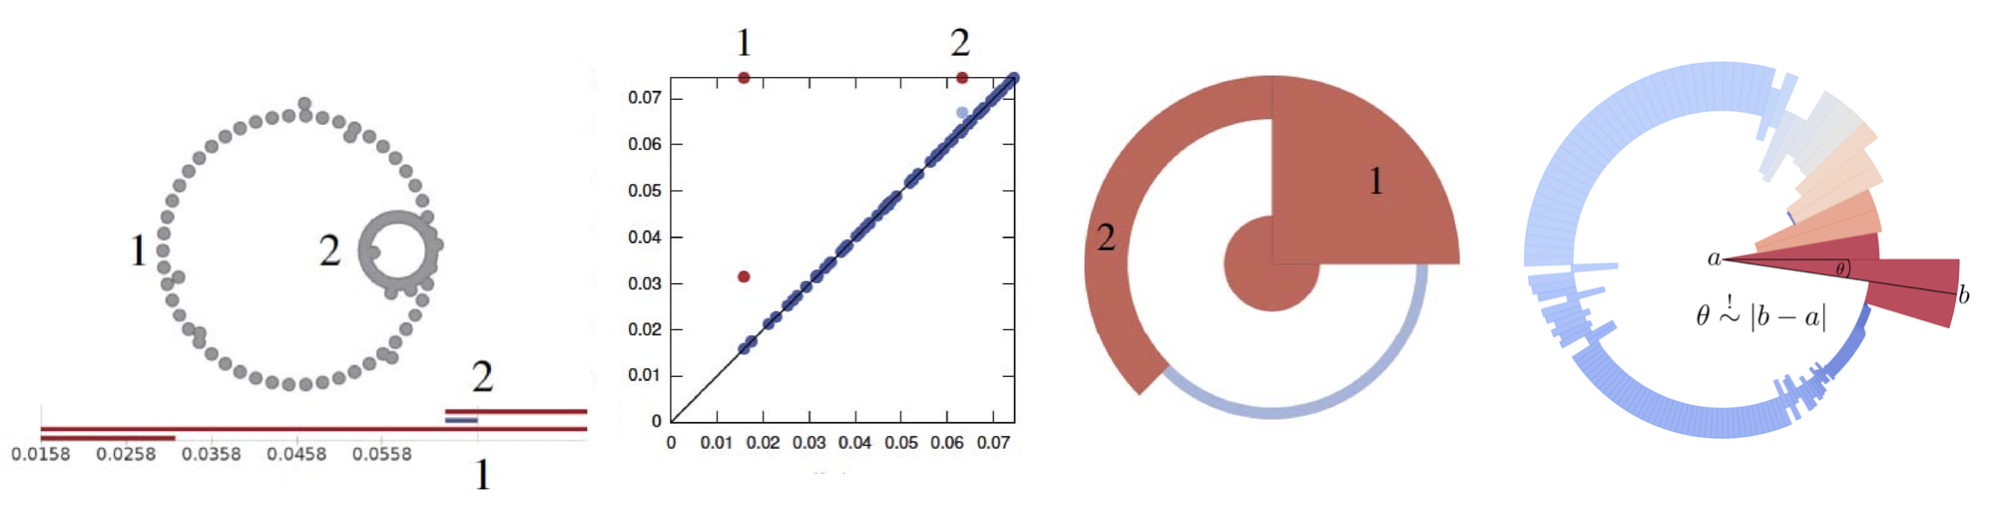
\includegraphics[width=\textwidth]{persistence_ring}
    \caption{Illustrative data set of two circles (all figures taken directly  from~\cite{rieck2012multivariate}). From the left to right, we have (1) the data set and it's persistence barcodes below it, (2) its corresponding persistence diagrams describing the significant 1-dimensional homology features (loops), (3) the persistence ring proposed by~\cite{rieck2012multivariate}, and (4) the persistence ring for a more complicated data set (not shown). The fourth figure illustrates the idea of the persistence ring: the angular distance $\theta$ of each portion of the pie chart represents the significance of a corresponding topological feature.}
    \label{fig:p_ring}
\end{figure*}

% Related Work
% - Identify at least 10 good references to discuss (6 beyond the pitch).
% - Focus primarily on current, relevant, peer-reviewed literature from  high-quality visualization research venues (Links to an external site.) such as IEEE VIS (InfoVis, VAST, SciVis), TVCG, CHI, EuroVis, and CGF.
% - The work most relevant to your project may be a technique applied in a different domain but that would be transferable to yours.
% - Cite and describe the relevance of these papers. You do not need to understand these papers in depth yet.
% - Make sure to focus on writing a narrative of how your project builds on and contrasts with prior work. This shouldn't just be a list of papers. This sections should help convince us that your project has the potential to make a research contribution.
\section{Related Work}
Although there has been much work done on visualizing graphs changing over time, but to the author's knowledge, such work is limited when it comes to visualizing simplicial complexes satisfying certain topological guarantees. One of the closest efforts in spirit to our own is the work of Suh et al.~\cite{suh2019persistent} or the work of Rieck et al.~\cite{rieck2012multivariate}\footnote{For a more visual explanation, see: \url{https://bastian.rieck.me/research/Vis2012_Slides.pdf}}, both published in the \emph{IEEE Transactions on Visualization and Computer Graphics}. The former discusses the use of persistent homology to guide a force-directed layout algorithm towards a producing a more topologically-accurate embedding of a graph, while the latter is aimed at visualizing the topological information (encapsulated through the use a \emph{persistence }) via a pie-chart-like graphic, which they call a \emph{persistence ring}. See Figure~\ref{fig:p_ring} for a visual graphic of persistence rings, as well as many other equivalent persistence representations. Other, more global visualization options for topological information include \emph{CROCKER}-stacks and \emph{vineyards}---see Xian et al. for an overview~\cite{xian2020capturing}. 

At the highest level of abstraction, homological persistence summarizes the topological features of a given data sets. The type of topological feature being summarized depends on the homological dimension chosen. The $0$-th dimensional homology classes characterize the connected components, or clusters, of a space; although this information can be conveyed using the above persistence rings, another possibility is to draw and augment the hierarchical constructions associated to these objects dynamically over time, see~\cite{oesterling2011visualization}, which was also published at the \emph{IEEE Transactions on Visualization and Computer Graphics}. 

% A popular set of tools for quantitatively understanding the more precise aspects of these methods is being pioneered y the field of Topological Data Analysis (TDA).

% A simplicial complex $K$ is a 


% TDA is a new(er) field of academia that is at the intersection of computational geometry, algebraic topology, and data science. Though the latter is, by now, a very interdisciplinary field with many methods that are both applied and theoretical, the former two have relatively deep theoretical foundations. These theoretical foundations play a significant role in characterizing the "goals" of data science at a very precise level, though such a level requires a certain amount of expertise that is not usually emphasized in the traditional data science curricula. This "bottom-heaviness" in theory can present a barrier to practitioners wanting to use such powerful theory. Thus, visualizations which help to demonstrate more clearly the intuition behind the theory may be invaluable to removing these barriers. 

% Network analsyis employs the uses of graphs to describe Graph-drawing, as of the time of writing, a well-studied field. 


% Despite their generaliz 


% Describe your target user(s). Who are they, what problems to they face, what data and tools do they use already? Also, who are you collaborating with outside the class (if anyone), with email addresses?
\subsection{Target Users and Collaborators}
We have no collaborators that we are working with. There are, however, a number of target user groups who may benefit from the work we do here. These include: 
\begin{enumerate}
    \item Users that use \texttt{R} or \texttt{Python} for data analysis 
    \item Applied researchers in TDA looking for ways to understand Persistence Homology
    \item Applied researchers in network visualization looking to understanding how certain topological properties of their data sets change over time
\end{enumerate}

% Explicitly identify what data you will be using for your project, or what data you will need to generate/collect. Hyperlink to it if possible.
\subsection{Data}
The initial data sets to demonstrate the fidelity of the methods we study in this effort will be derived synthetically from parameterized families of generative models. The particular type of generative model is often coupled to domain of application. For example, while the study of swarm or flock behavior is often employed with linearly-parameterized functions such as \emph{boid simulations}~\cite{reynolds1987flocks}, other types of physical simulations (e.g. time-varying dynamical systems) are generated by identifying an underlying systems of differential equations that accurately captures the systems observed behavior~\cite{kim2021spatiotemporal}. While we intend to identify specific applications (and thus particular types of generative models), it's important to emphasize that the methods we study in this effort are domain-independent. 

It's worth noting that TDA, as a field, has already made much headway in helping scientists and applied researchers understand significant topological features in their data. From aiding the analysis of pedogenetic properties of European topsoil~\cite{savic2017topological} to extracting latent brain structure from complex fMRI data~\cite{salch2021mathematics} to characterizing the flocking behavior of biological aggregations models~\cite{topaz2015topological}---TDA is replete with a vibrant community of domain experts that stand to benefit from extensions made by the visual data science community. 


% Describe what you plan to do and what technologies you'll need. Also detail any preliminary work that exists. Note that you need not have done preliminary work, but if you have include details and images here.
\subsection{Execution Plan \& Preliminary Work}
Aside from the research we have done, we have no preliminary work done thus far. 

Our current plan is to start by understanding more in-depth the persistence-augmented force-directed algorithm developed by Suh et al.~\cite{suh2019persistent}, and to replicate some of their results using either a Python or Javascript library well adapted to the visualization of force-directed graphs. Once this has been implemented, we will see if its possible to extend both the algorithm and the software to support higher dimensional complexes beyond graphs. Note that, as these complexes are drawn in $\mathbb{R}^2$, extending existing software to support drawing arbitrary polygons is enough for this task (though the theoretical extension to incorporate forces from $d$-simplices will require some additional work). 

Given a dynamically drawn complex, there are several options available for visualizing the persistence information; these include anything from persistence \emph{diagrams}, persistence \emph{barcodes}, persistence \emph{landscapes}, etc. (again see~\cite{chazal2021introduction} for an overview). Extending D3.js's tools (or some other JS library) support persistence \emph{rings}~\cite{rieck2012multivariate} would perhaps be the most suitable visualization for the dynamic setting. This simply requires adapting a variation of a pie chart to the time-varying setting, such that the [angular] partitions of the chart can expand or shrink dynamically. 

Finally, it's worth noting that the first author has experience creating and binding modern JS libraries to high-level languages like \texttt{R}\footnote{See the source code for the \texttt{pixiplex} package\url{https://github.com/peekxc/pixiplex}.}, so the first task couple of tasks is considered plausible in the given time constraints. 

\bibliographystyle{abbrv-doi}
\bibliography{template}

\subsection{Group Charter}
% Group Purpose: State the reasons for this group's formation and the group's purposes. Who are your stakeholders / intended users, and what are their expectations of and for the group? (You don't need to reiterate details in the proposal, just anything additional.)
\noindent 
\textbf{Group Purpose:} The groups purpose is to understand the current state of the art for visualizing networks (i.e. complexes) in dynamic settings. Primarily, the purpose of this group is to advance this state of the art towards making these dynamic network visualizations more explainable and accessible to the general user. Our expectations are to work towards something we both find interest in. 
\\
\\
% Group Goals: What are the group's project, process, and quality goals? To what level of performance are group members willing to commit, and what course grade are you collectively aiming for? Articulating these goals will make a difference in your group's performance.
\noindent
\textbf{Group Goals:}
Our group goals are essentially to learn as much new material related to the project in the desired time frame. Related to presentation and quality, our goal is to present what we learn in as simple and accessible a manner as possible. The technical merit of our project will be judged independently of this group charter.
\\
\\
% While some group responsibilities are shared by all members, collaborative groups work best when members also have unique roles and responsibilities. These could be technical and/or project management related, e.g., group leader, meeting facilitator, documentation coordinator, information manager, point person for sponsor/advisor communications, etc. Consider these assignments carefully.
\noindent
\textbf{Group Member Roles/Responsibilities:} Matt will take a lead on the technical aspect of the project while Ayub will focus on project management. 
\\
\\
% How and when will this group meet? What are the norms and ground rules the group will agree to? How will you conduct discussions and make decisions? How will you handle dissenting views among members? How will you hold each other accountable for living by these rules and for task completion? What kind of participation and level of commitment do you expect from one another?
Start on time.
Practice respect for yourself and others.
Come prepared to do your part.
Be a good listener.
No put-downs.
Make sure everyone gets a chance to contribute or speak.
Accept constructive criticism gracefully.
Critique ideas, not people.
Stay on task.
No interruptions; let people finish talking.
Ask for help when you’re confused about what to do.
Help others when you can.
Do your fair share of the work.
\\
\\
\noindent
\textbf{Ground Rules:} We will meet weekly to discuss project timeline. We will ideally meet in person, but go virtual if needed. We expect to come prepared to these meetings with previous tasks completed. We want to make sure everyone have a chance to contribute and/or speak. When someone is speaking, let them finish talking without interrupting. Moreover, critique ideas and not people. We hope to divide up tasks equally, check in on progress, and make necessary adjustments on a week to week basis. We will conduct discussions in person and try to find common ground when making decision. We will hold each other accountable by having specific assigned tasks due before our meeting. We expect a high level of commitment and communication from one another. 
\\
\\
% What barriers to effective group work might potentially arise in the course of completing your project and other group obligations, and how will you handle them if they materialize? What problems with group dynamics have you experienced in the past, and how will you handle them if they come up again?
\noindent
\textbf{Potential Barriers and Coping Strategies:}
We will solve any barriers or conflicts to effective group work by compromising when necessary and by treating each other with respect. These barriers could include things like difference of opinion, target application, and approach. Our plan to handle these barriers are to use conflict-resolution to come to a mutual understanding such that the project can proceed. 
\\
\\



\end{document}
